\chapter{Mediciones de Luminosidad y Afterglow}
\label{ch3}

La medición precisa de la luminosidad suministrada al experimento CMS por el LHC es fundamental por varias razones. En tiempo real, la medición de la luminosidad ofrece información sobre el rendimiento del LHC y CMS, incluyendo el monitoreo de las tasas de activación de los disparadores. En el análisis fuera de línea, la luminosidad es un componente clave para calcular la sección eficaz de los procesos observados o para establecer límites superiores en la búsqueda de procesos más allá del modelo estándar.

Como se ha mencionado, para medir la luminosidad en CMS se utilizan un total de siete luminómetros, cada uno de los cuales mide una cantidad específica en el detector, como impactos, trazas o cúmulos. La tasa $R$ medida por el luminómetro es proporcional a la luminosidad instantánea $\mathcal{L}_{inst}$ , con una constante de proporcionalidad dada por la sección eficaz visible $\sigma_{vis}$.

\begin{equation}
R(t)=\mathcal{L}_{inst}\sigma_{vis}
\label{lumi_exp_gen}
\end{equation}

La determinación de \( \sigma_{\text{vis}} \) se realiza mediante escaneos de van der Meer (vdM) utilizando una configuración especial del LHC.

\section{Pixel Cluster Counting method (PCC)}

El método PCC utiliza el número promedio de cúmulos (clústers) de píxeles en el detector de píxeles de silicio del CMS para determinar una medición de luminosidad offline. Este método aprovecha la alta densidad de píxeles en la región interna del sistema de rastreo de CMS. Esto significa que la probabilidad de que un solo píxel sea impactado por dos partículas cargadas provenientes del mismo cruce de haces es extremadamente baja. Esta gran granularidad y baja ocupación proporcionan mediciones con una excelente respuesta lineal respecto al pile-up (número de interacciones por cruce de haces) $\mu$. En promedio, la ocupación del detector es inferior al 0.1\%\cite{lumi_precise_2015_2016}.\\

La Figura 3.1 muestra una simulación con eventos de colisión $pp$ de cero sesgo, en la que se presenta la tasa de conteo de clústers de píxeles como una función del pile-up en el rango observado en la Run 2, que va de 0 a aproximadamente 50 $\mu$. El número promedio de clusters de píxeles es del orden de 111 por evento. La curva roja es un ajuste polinomial de primer orden con pendiente. Los resultados indican un alto nivel de concordancia, evidenciado por el ajuste estimado de bondad de ajuste $\chi^{2}$  por grado de libertad (dof), de aproximadamente 0.5, lo que demuestra que la tasa PCC es altamente lineal en este rango bajo condiciones simuladas \cite{ Phase2_Upgrade,lumi_precise_2015_2016}.

\begin{center}
  \begin{figure}[h!]
    \centering
    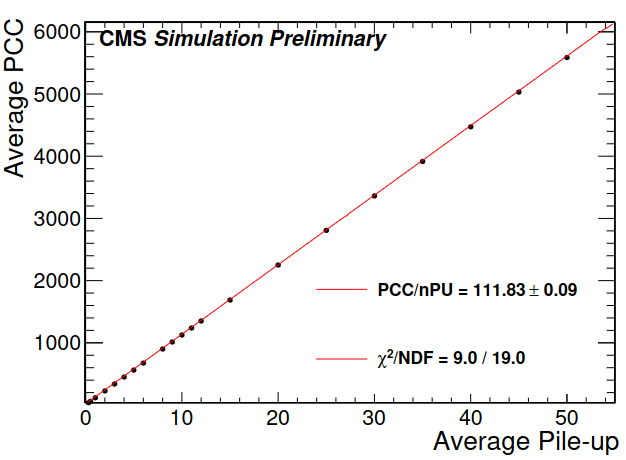
\includegraphics[scale=.35]{Chapter3/pileup_lineality.png} 
    \caption[Linealidad del PCC con pile-up]{ Linealidad del conteo de clústers de píxeles en el rango de pile-up observado en la Run 2 (de 0 a aproximadamente 50) a partir de simulaciones. La línea roja es un ajuste lineal a los puntos.}
    \label{pileup}
  \end{figure}
\end{center}

Para obtener el número promedio de clústers de píxeles por evento, se promedian varios eventos de cero sesgo. Este valor se define como::

\begin{equation}
\left < N_{\text{cluster}} \right > \equiv \left < N_{\text{cluster}/\text{interaction}} \right > \mu
\end{equation}

Bajo condiciones de sesgo mínimo, $\mu$ se puede expresar como: 

\begin{equation}
\mu = \frac{\sigma_{\text{minBias}}}{f} \cdot \mathcal{L}_{inst}
\end{equation}

donde $f$ es la frecuencia de revolución del LHC y $\mathcal{L}_{inst}$ es la luminosidad instantánea de un solo paquete (SBIL, por sus siglas en inglés). La sección eficaz de sesgo mínimo ($\sigma_{text{minBias}}$) está relacionada con la sección eficaz visible del PCC mediante el número promedio de clústers por interacción:

\begin{equation}
\sigma_{vis}= \left < N_{\text{cluster}/\text{interaction}} \right >\cdot \sigma_{\text{minBias}}
\end{equation}

Juntando todo, la luminosidad obtenida será:

\begin{equation}
\mathcal{L}_{inst}=\frac{\left < N_{\text{cluster}} \right >}{\sigma_{vis}} \cdot f
\end{equation}

%This method is capable of providing a precise luminosity measurement over longer time periods, but it cannot do so for a single luminosity section (23 seconds) as is possible with online luminometers. The reason for this limitation is the limited CMS trigger bandwidth available for collecting data \cite{pas_18}. A detailed discussion on this topic can be found in the next chapter.\\

%PCC si calcula lumi por cada lumi section.  Esto no tiene que ver con online vs offline.  PCC es un offline luminometro, quiere decir que los datos llegan tarde.  Con PCC solo podemos calcular lumi cada lumi section, debido a la baja estadistica (por la lectura de los datos de zero bias).  otros luminometros tienen precision con NB4 (HF, PLT, BCM1F).  


\section{Datos adquiridos en 2022}

El 12 de julio de 2022, comenzó la recolección de datos para Run 3 del Gran Colisionador de Hadrones (LHC), lo que resultó en una luminosidad total registrada de 38.48 fb⁻¹ durante ese año. Estos datos se recolectaron durante colisiones protón-protón con una energía en el centro de masa de √s = 13.6 TeV. El periodo de recolección de datos comenzó con el inicio de los haces estables y concluyó cuando el haz fue detenido intencionalmente o cuando se interrumpieron los haces estables momentáneamente para realizar estudios del haz. La luminosidad entregada por el LHC al CMS (representada en azul) y la luminosidad registrada por CMS (mostrada en naranja) durante este periodo se ilustran en la Figura 3.2 \citep{wikicern}.

\begin{center}
  \begin{figure}[h!]
    \centering
    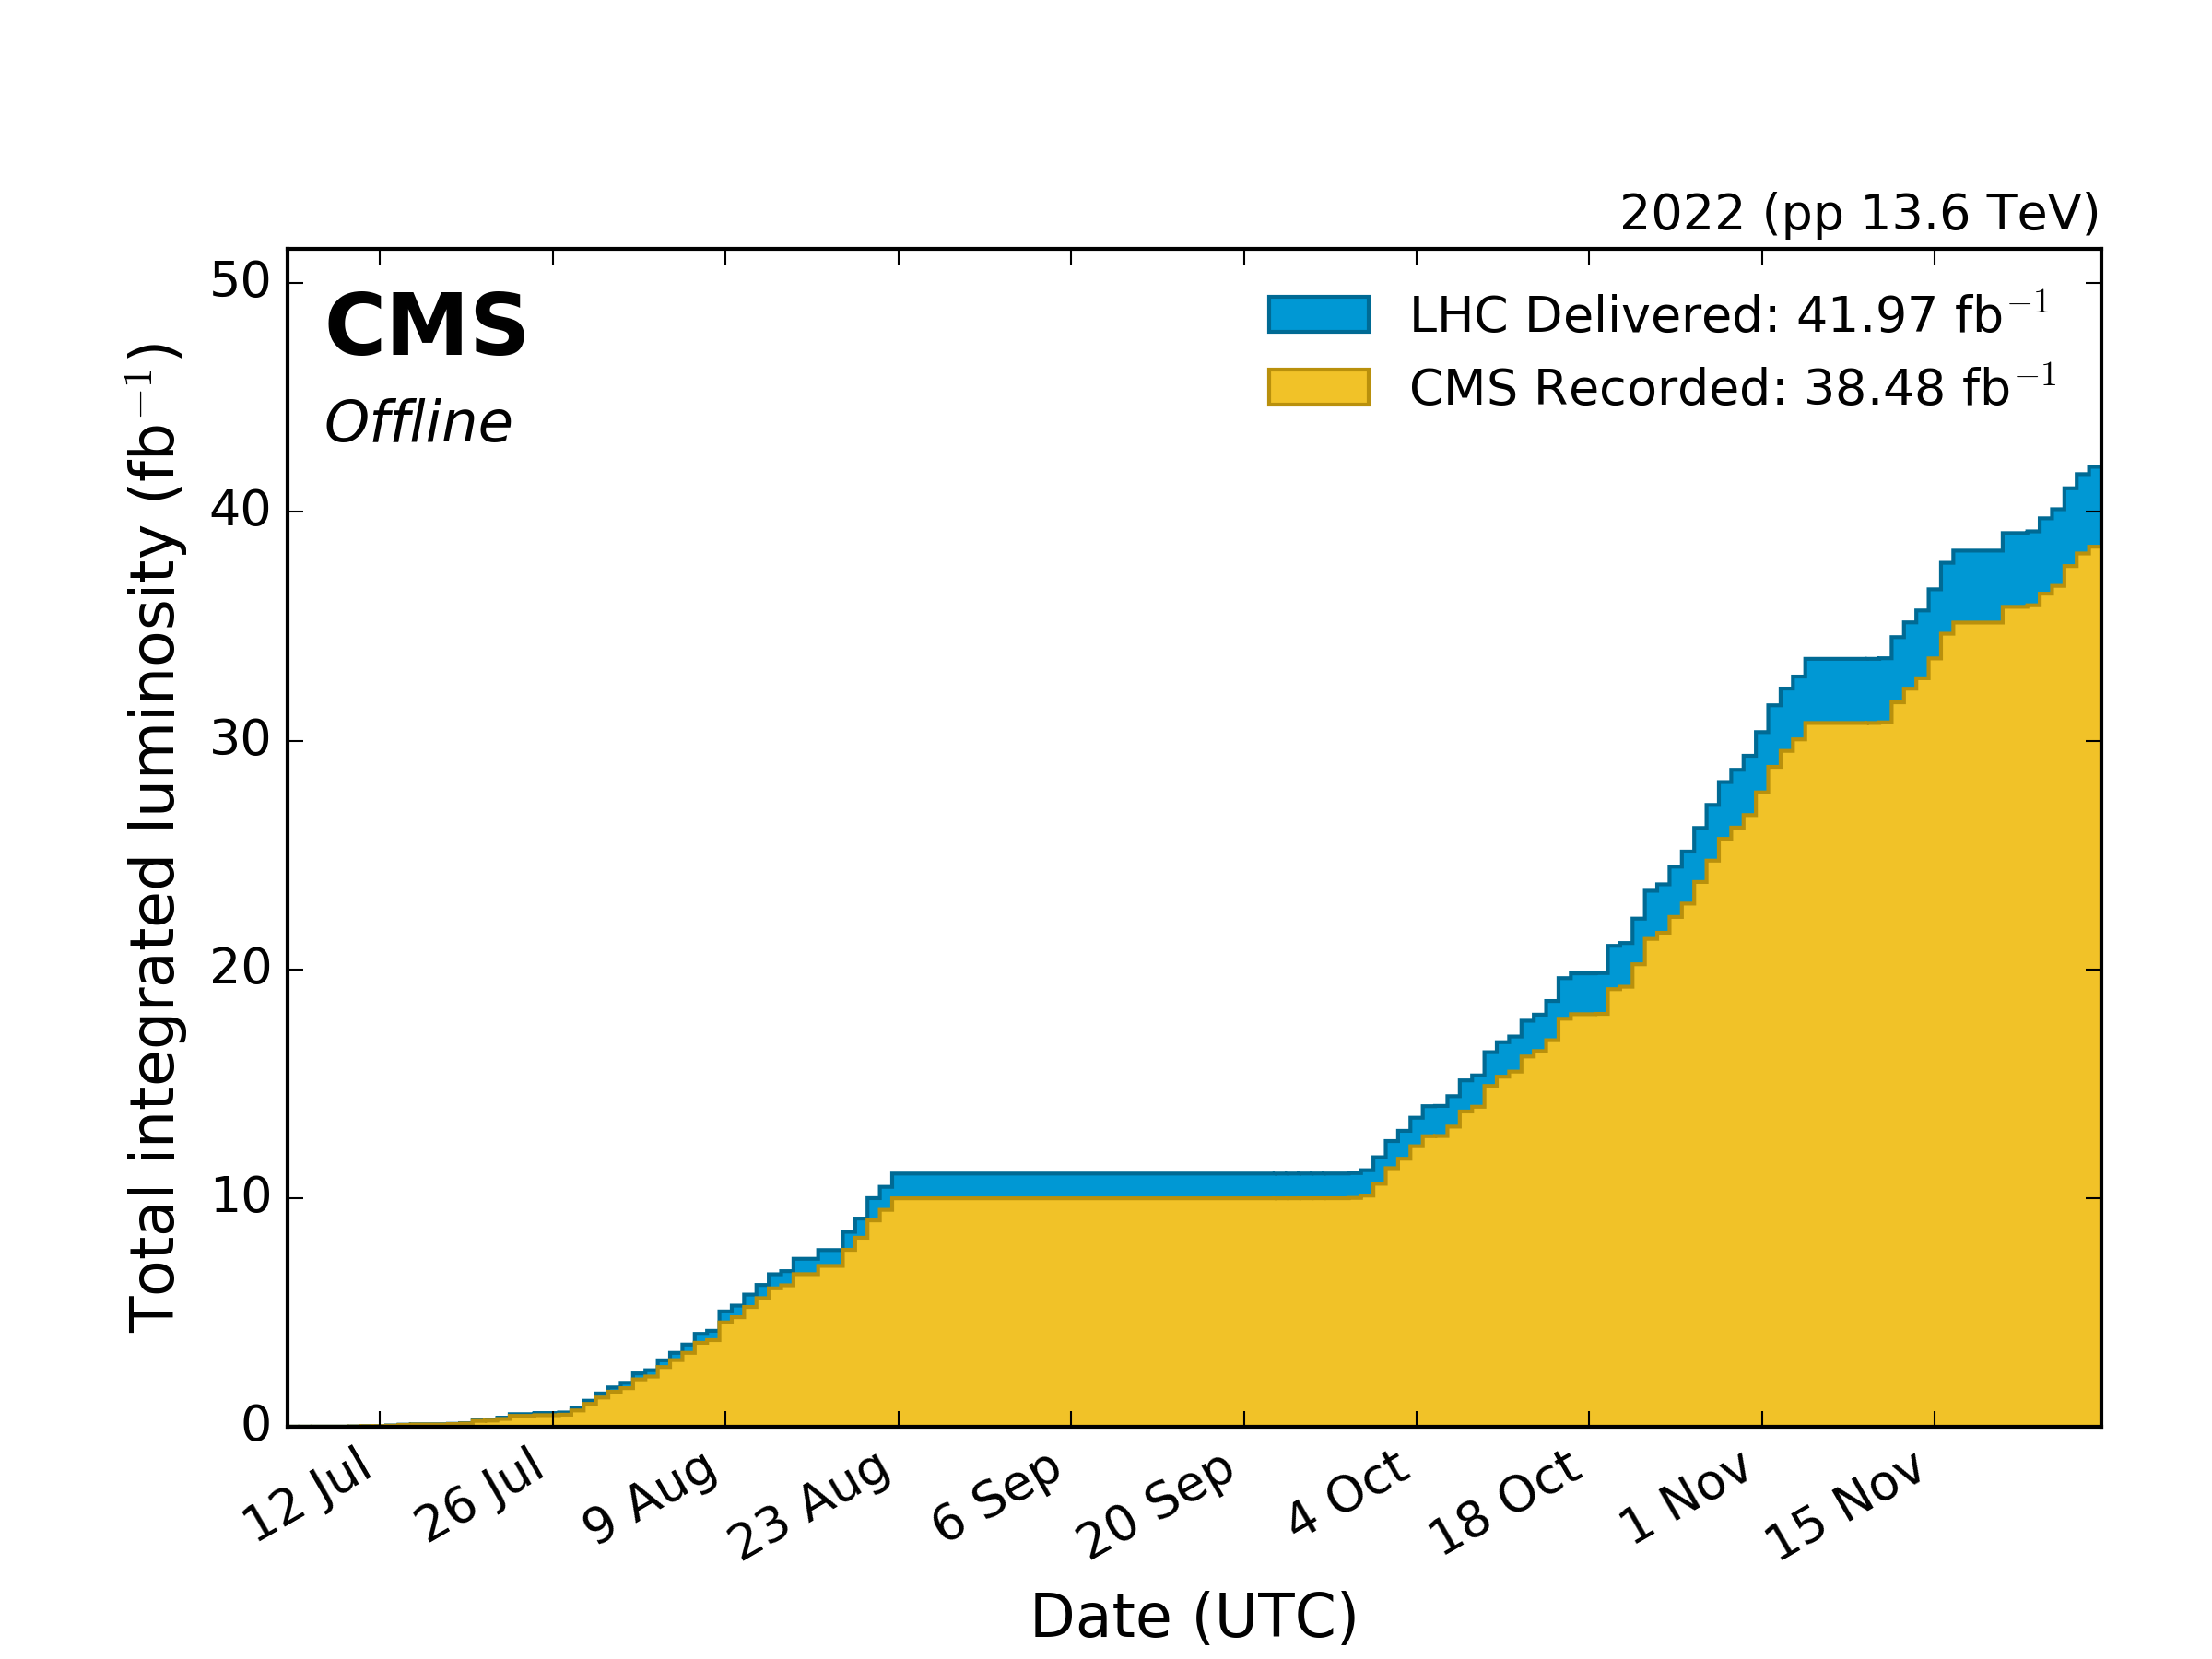
\includegraphics[width=.45\textwidth]{Chapter3/lumi_per_day_cumulative_pp_2022.png}
    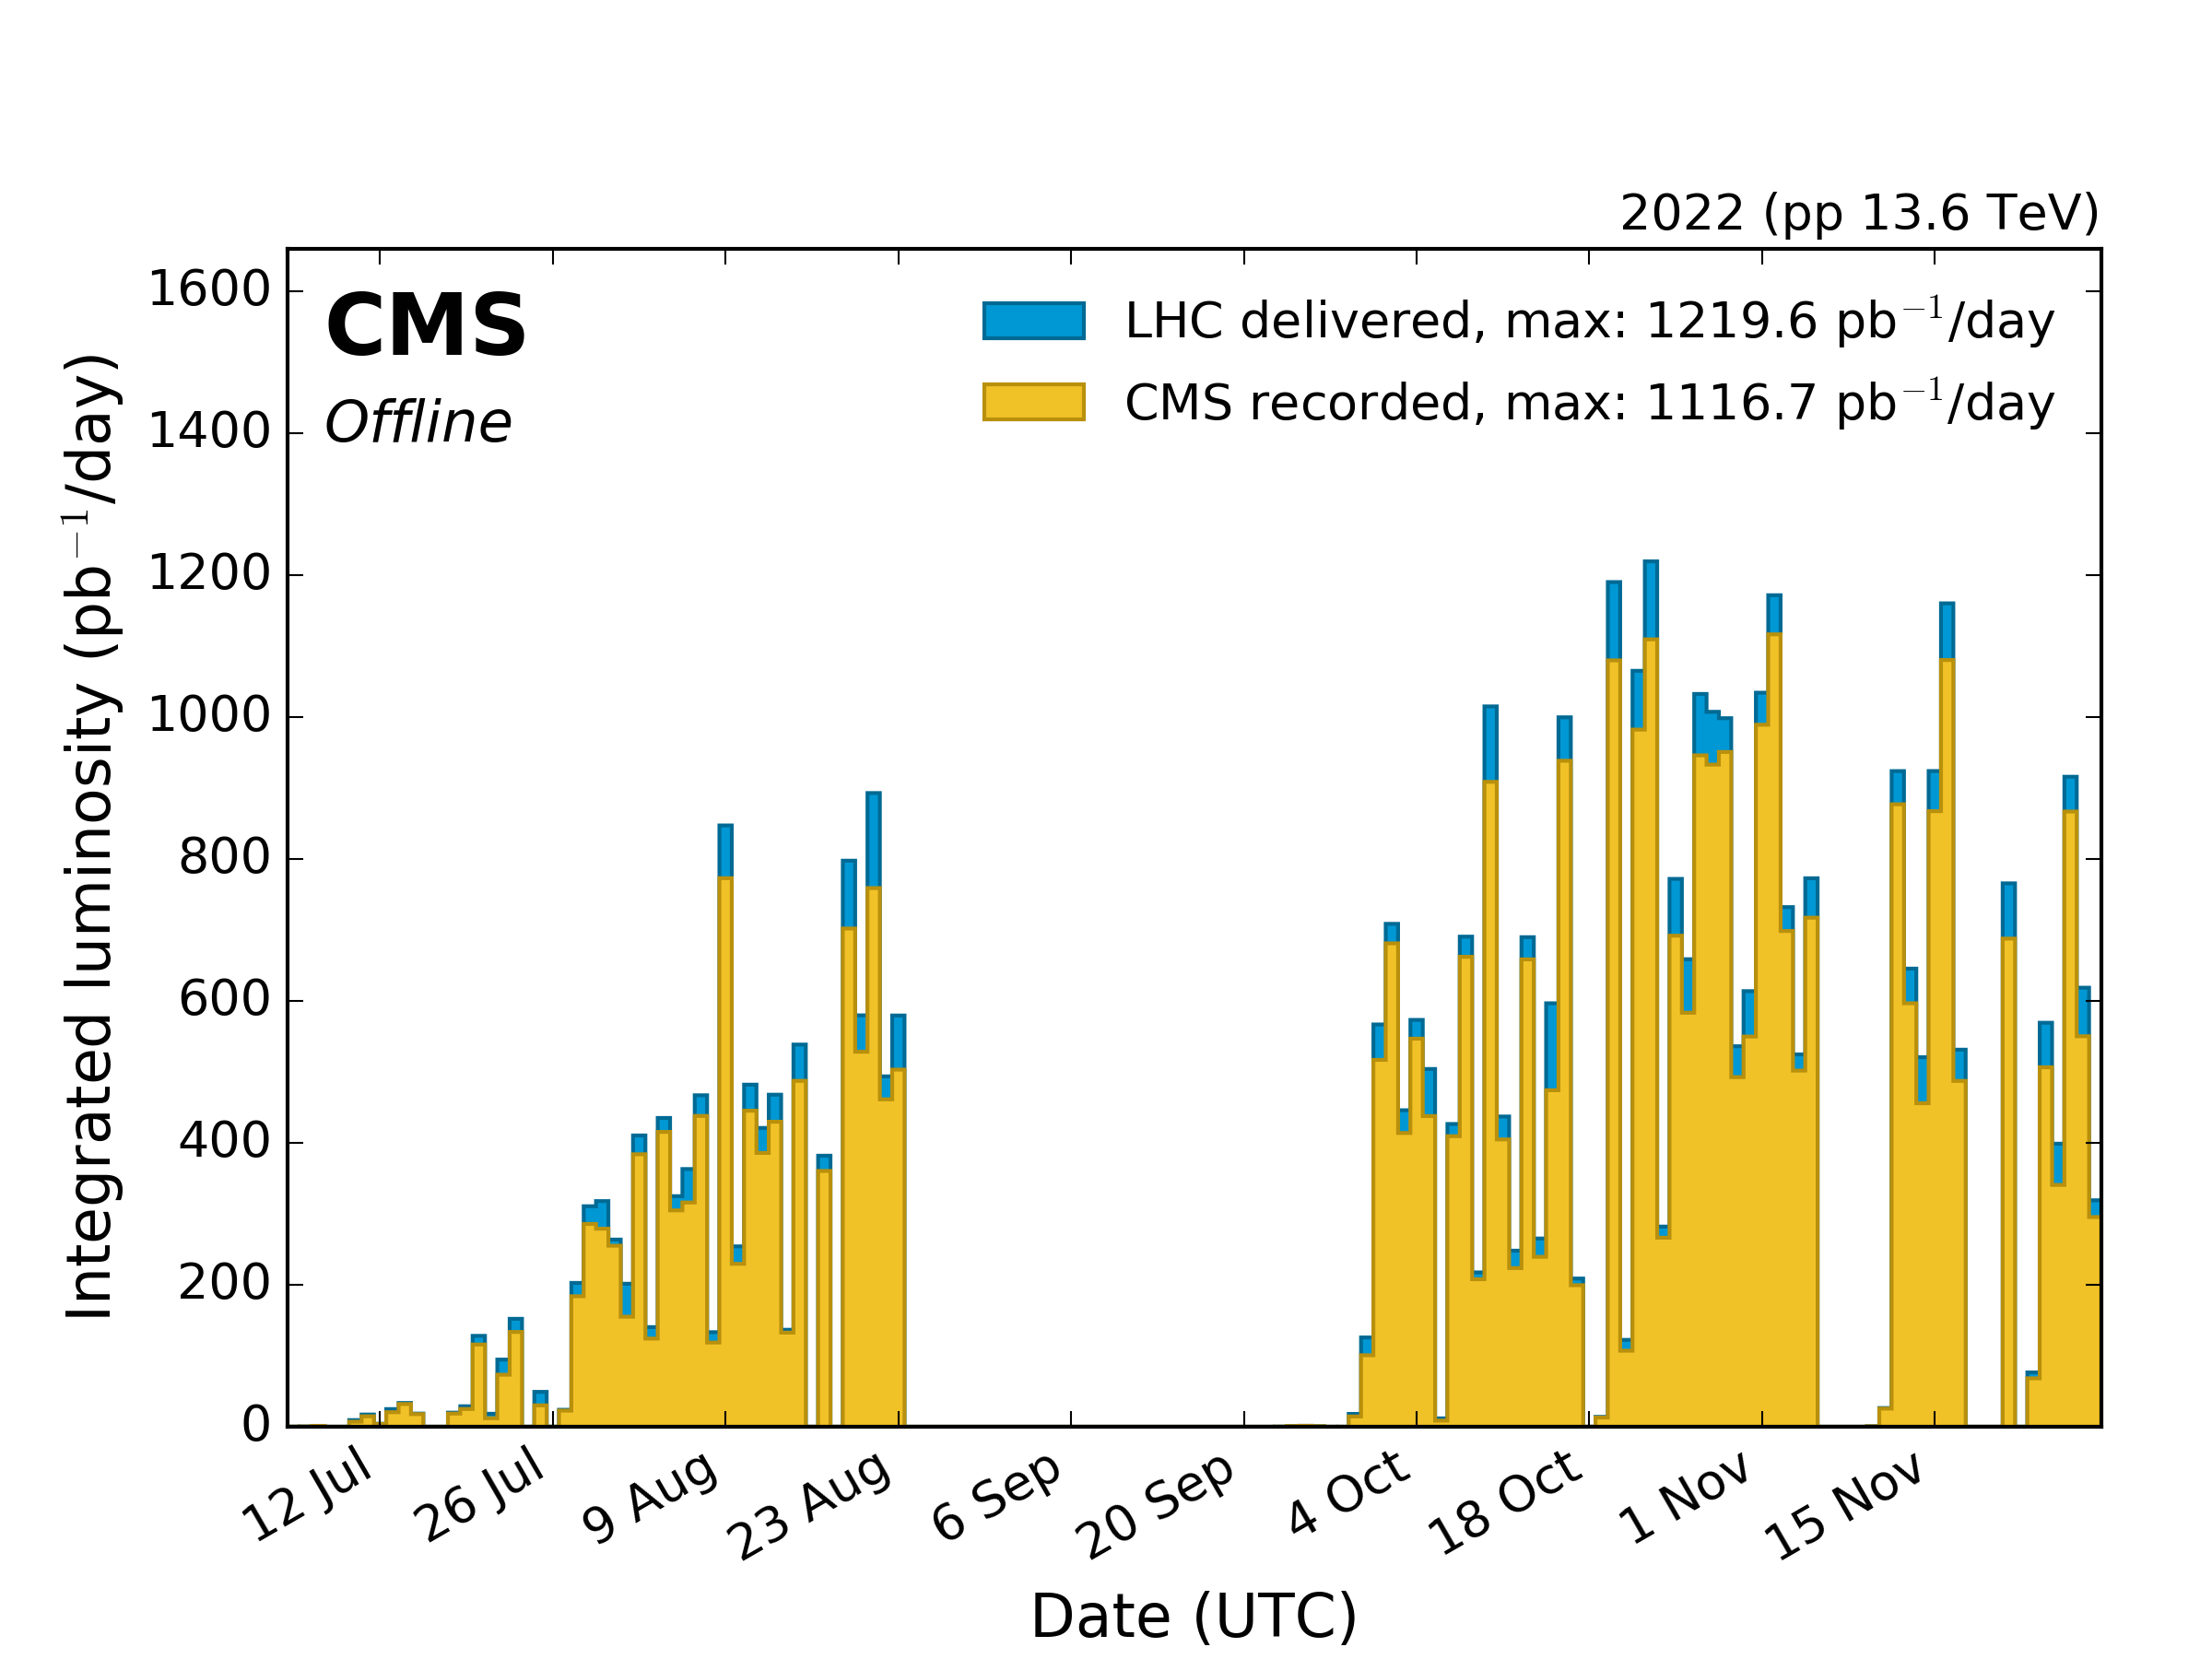
\includegraphics[width=.45\textwidth]{Chapter3/lumi_per_day_pp_2022.png}
    \caption[Luminosidad integrada acumulada día a día en 2022]{(izquierda) Luminosidad integrada acumulada día a día. (derecha) Luminosidad integrada día a día en 2022, como el primer gráfico, pero no acumulativa.} 
    \label{Lumi_2022}
  \end{figure}
\end{center}


\section{PCC sobre la orbita del LHC}

En esta sección se presenta el análisis del Pixel Cluster Counting (PCC) a lo largo de toda la órbita del LHC, que comprende 3564 espacios disponibles para colisiones (buckets). El objetivo es estudiar cómo varía el conteo de cúmulos de píxeles en función de la posición de las interacciones dentro de la órbita y analizar la estructura específica de los trenes de protones y las secciones vacías entre ellos.\\

El LHC no utiliza todos los espacios disponibles para colisiones de manera continua; en su lugar, los protones se agrupan en lo que se conocen como trenes. Cada tren está compuesto por una serie de bunches o "vagones", que son grupos de protones que circulan de manera sincronizada alrededor del anillo del acelerador. Entre estos trenes existen espacios vacíos llamados gaps, que se emplean para evitar la superposición de señales no deseadas y permitir la estabilidad del sistema de inyección de los haces.\\

La gráfica obtenida (Figura 3.3) muestra el número de clusters de píxeles contados por el sistema PCC a lo largo de toda la órbita del LHC, lo cual incluye tanto las regiones donde ocurren colisiones como las regiones de espacio vacío donde no hay interacciones. En la gráfica, los trenes de protones son claramente identificables como picos que se agrupan en ciertas regiones, mientras que las secciones vacías entre los trenes aparecen como caídas abruptas en el conteo de clusters.\\

En la gráfica, los trenes de protones son observados como series de bunches sucesivos que producen un alto número de cúmulos de píxeles en el detector de CMS. A medida que el haz de protones interactúa con los bunches, los cúmulos de píxeles detectados aumentan significativamente debido a las colisiones de partículas dentro del detector.\\

Los gaps son esenciales para prevenir la acumulación excesiva de efectos indeseables, como el afterglow o el ruido residual, y garantizar un funcionamiento estable del sistema de inyección y detección.\\

\begin{center}
  \begin{figure}[h!]
    \centering
    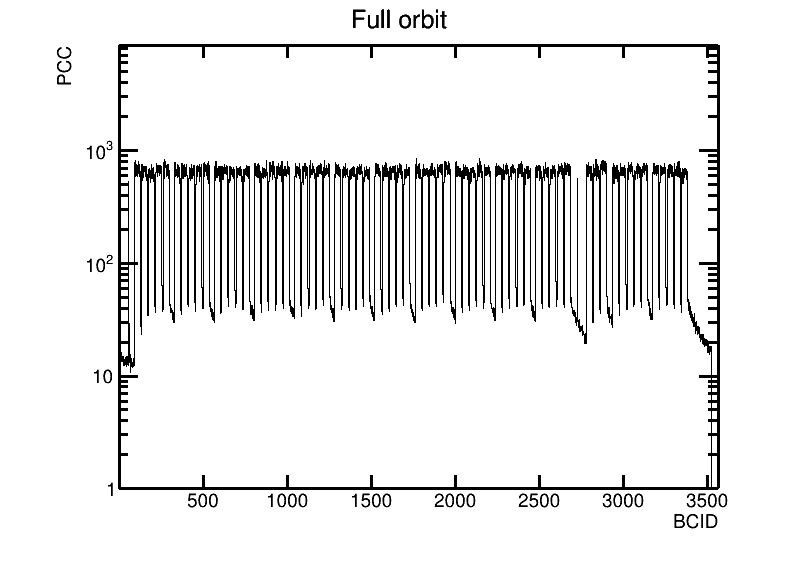
\includegraphics[width=.55\textwidth]{Chapter3/full_orbit_data_only_no_fit.png}
    \caption[Llenado (fill) de una orbita]{Se presenta el número de clusters de píxeles contados por el sistema PCC a lo largo de toda la órbita del LHC, mostrando la estructura de trenes y gaps entre bunches.} 
    \label{Lumi_2022}
  \end{figure}
\end{center}

Esta gráfica es fundamental para visualizar cómo se distribuyen las colisiones y los espacios vacíos a lo largo de la órbita, lo que permite comprender mejor la estructura de los bunches y el impacto de los trenes en el conteo de cúmulos de píxeles.\\

\section{Observación del Afterglow}

En la Figura 3.4 se presenta un tren de bunches con la medición del número de clusters de píxeles detectados por el método PCC a lo largo de un tren de bunches en la órbita. En este caso, se puede observar el fenómeno conocido como afterglow, que afecta las mediciones posteriores a los bunches principales debido a la persistencia de señales residuales en el detector. Este afterglow se divide en dos tipos:\\

El \textbf{afterglow de tipo 1} es el resultado de un desbordamiento de la señal electrónica de un bunch crossing ID (BCID) al siguiente. En otras palabras, la señal medida en un bunch es afectada por un rezago de la señal electrónica de bunches anteriores. Este fenómeno es notable en la caída abrupta de las mediciones de PCC justo después de los bunches activos, tal como se muestra en la gráfica. La contribución del afterglow tipo 1 es predominantemente electrónica y tiene una caída rápida en los bunches inmediatamente posteriores al bunch principal.\\

El \textbf{afterglow de tipo 2} proviene de partículas secundarias generadas por la activación del material circundante debido a las interacciones del haz principal. Estas partículas tienen vidas medias más largas y decaen exponencialmente con el tiempo, lo que genera una señal residual en bunches posteriores durante un intervalo de tiempo más extenso. A diferencia del afterglow tipo 1, la caída del afterglow tipo 2 es más gradual, y está presente a lo largo de un rango más amplio de BCIDs, como se observa en la gráfica en bunches posteriores a los 40 BCID.\\

\begin{center}
  \begin{figure}[h!]
    \centering
    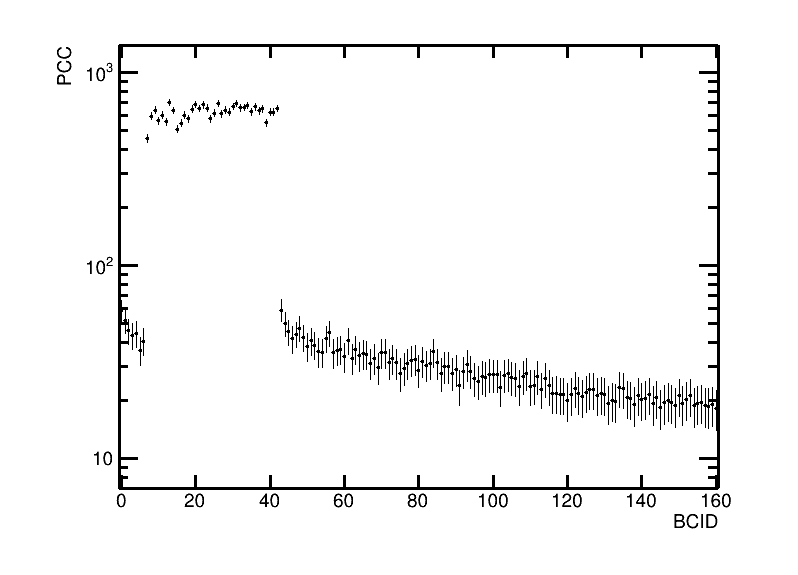
\includegraphics[width=.55\textwidth]{Chapter3/singleTrainNoFit.png}
    \caption[Gráfica de un tren]{La gráfica permite visualizar claramente ambos tipos de afterglow: el afterglow tipo 1 es visible en la caída abrupta en los primeros BCIDs (cerca del BCID 40), mientras que el afterglow tipo 2 se manifiesta como una disminución exponencial más suave a lo largo de los bunches posteriores (más allá del BCID 40).} 
    \label{Lumi_2022}
  \end{figure}
\end{center}

\section{Ajuste de Datos y Residuos}

Para ajustar los datos obtenidos en la medición del número de clusters de píxeles detectados, se utiliza un modelo compuesto que describe tanto el fenómeno de afterglow de tipo 1 como el de tipo 2, así como la contribución residual de interacciones previas. El modelo que se emplea para el ajuste de los datos está dado por la siguiente expresión analítica:

\[
f(x) = \sum_{k=0}^{N-1} n_k \left[ \delta_{x, x_k} + A \cdot \delta_{x, x_k + 1} + B_k \cdot e^{-C_k(x - x_k)} \cdot \Theta(x - x_k) \right] + D \cdot e^{-E \cdot x}
\]

Donde los términos son definidos de la siguiente manera:

\begin{itemize}
    \item $\delta_{x, x_k}$: Delta de Kronecker, que representa un pico en la medición exactamente en $x_k$, correspondiente a la señal principal del bunch colisionante.
    \item $A$: Amplitud del afterglow tipo 1, que es constante para todos los BCIDs.
    \item $\delta_{x, x_k + 1}$: Delta de Kronecker que representa el afterglow tipo 1 en el BCID inmediatamente siguiente ($x_k + 1$).
    \item $B_k$: Amplitud del afterglow tipo 2, que describe el decaimiento exponencial debido a la generación de partículas secundarias por activación del material circundante.
    \item $C_k$: Tasa de decaimiento exponencial del afterglow tipo 2.
    \item $\Theta(x - x_k)$: Función escalón de Heaviside, que asegura que el decaimiento exponencial del afterglow tipo 2 solo se aplique para $x \geq x_k$.
    \item $D$: Amplitud del ruido residual.
    \item $E$: Tasa de decaimiento exponencial del ruido residual.
\end{itemize}

Este modelo compuesto tiene en cuenta tanto las contribuciones puntuales de los bunches colisionantes como el comportamiento más gradual del afterglow tipo 2, además de la influencia de colisiones previas que pueden generar señales persistentes en el detector.

A continuación, se presenta un ajuste de los datos experimentales utilizando este modelo. En la Figura 3.5, se observa el resultado del ajuste realizado a los datos obtenidos mediante el método Pixel Cluster Counting (PCC). El ajuste incluye tanto los picos asociados al afterglow de tipo 1, como las contribuciones del afterglow tipo 2 y la componente residual de interacciones previas.

\begin{center}
  \begin{figure}[h!]
    \centering
    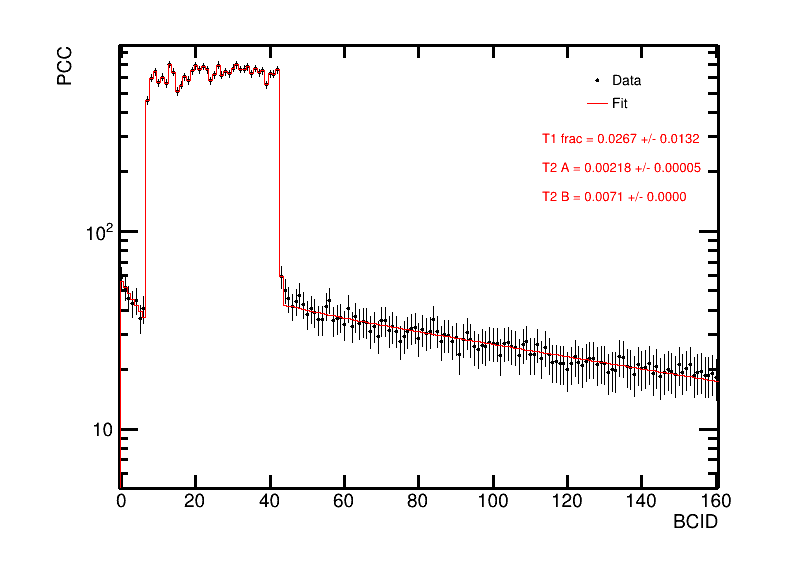
\includegraphics[width=.55\textwidth]{Chapter3/fitAfterglowTrain_fit.png}
    \caption[Ajuste de los Datos Experimentales]{ Ajuste de los datos obtenidos mediante el método Pixel Cluster Counting (PCC) utilizando el modelo compuesto que incluye las contribuciones del afterglow tipo 1, tipo 2 y residual. Los parámetros $A_{k}$, $B_{k}$, $C_{k}$, $D$ y $E$ son ajustados a los datos experimentales, mostrando cómo el modelo describe las señales detectadas a lo largo de los bunches.} 
    \label{Lumi_2022}
  \end{figure}
\end{center}

Por otro lado, se muestran los residuos del ajuste en la Figura 3.6, que representan la diferencia entre los datos observados y el modelo ajustado. Estos residuos permiten evaluar la calidad del ajuste y detectar posibles desviaciones o inconsistencias en la modelización de los datos.

\begin{center}
  \begin{figure}[h!]
    \centering
    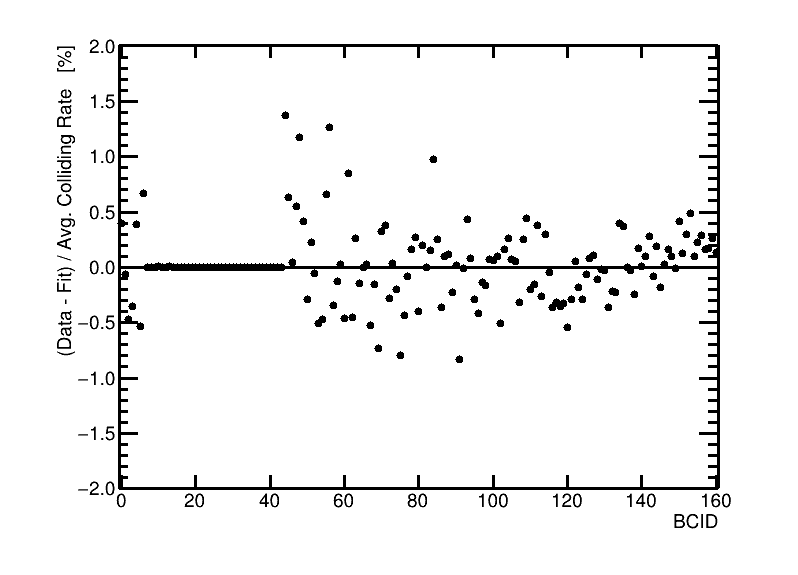
\includegraphics[width=.55\textwidth]{Chapter3/fitAfterglowTrain_residuals.png}
    \caption[Residuos del Ajuste]{Residuos del ajuste realizado a los datos experimentales, representando la diferencia entre los datos observados y el modelo ajustado. Los residuos se distribuyen alrededor de cero, lo que indica la calidad del ajuste y la capacidad del modelo para capturar las características del fenómeno observado.} 
    \label{Lumi_2022}
  \end{figure}
\end{center}

El análisis de los residuos es fundamental para asegurar que el modelo propuesto sea adecuado para describir el comportamiento del afterglow en los datos experimentales. Los residuos deben distribuirse de manera aleatoria alrededor de cero, sin patrones sistemáticos, lo que indicaría que el modelo ha capturado de manera adecuada las características del fenómeno observado.

\section{Evolución de los Parámetros en Función del Tiempo}

En esta sección, se presenta un análisis de la evolución temporal de los parámetros del modelo matemático utilizado para ajustar los datos obtenidos mediante el método de conteo de clusters de píxeles (Pixel Cluster Counting, PCC). Como se describió en la sección 3.5, el modelo matemático empleado para el ajuste de los datos incluye contribuciones del afterglow tipo 1, tipo 2 y una componente residual de interacciones previas. Los parámetros clave del modelo son \(A\), \(B_k\), \(C_k\) y \(E\), cuyas propiedades ya fueron definidas en la sección anterior.

Para analizar la evolución de estos parámetros en función del tiempo, se realizó un ajuste de los datos utilizando el modelo descrito en la sección 3.5. Los valores de los parámetros \(A\) y \(B_k\) se obtuvieron para diferentes momentos durante la toma de datos, lo que permitió graficar su comportamiento a lo largo del tiempo.

\begin{figure}[h!]
    \centering
    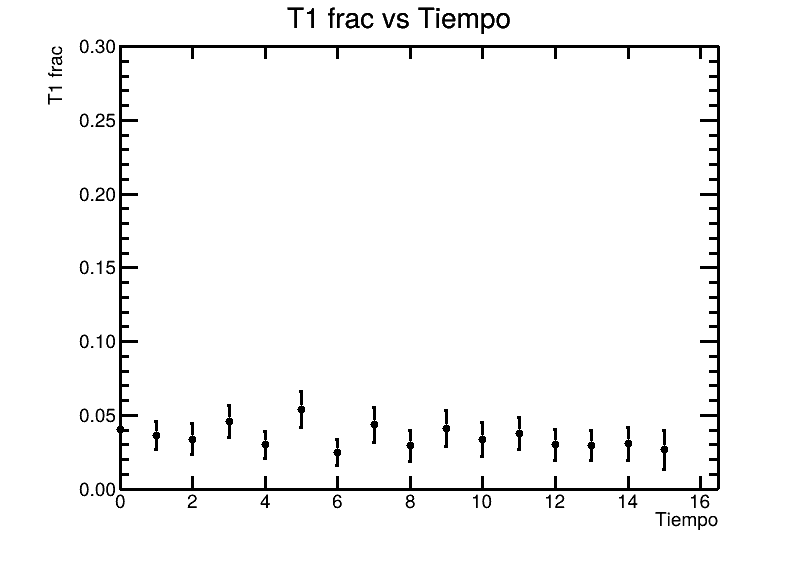
\includegraphics[width=.4\textwidth]{Chapter3/T1F_vs_tiempo.png}\hspace{0.1 cm}     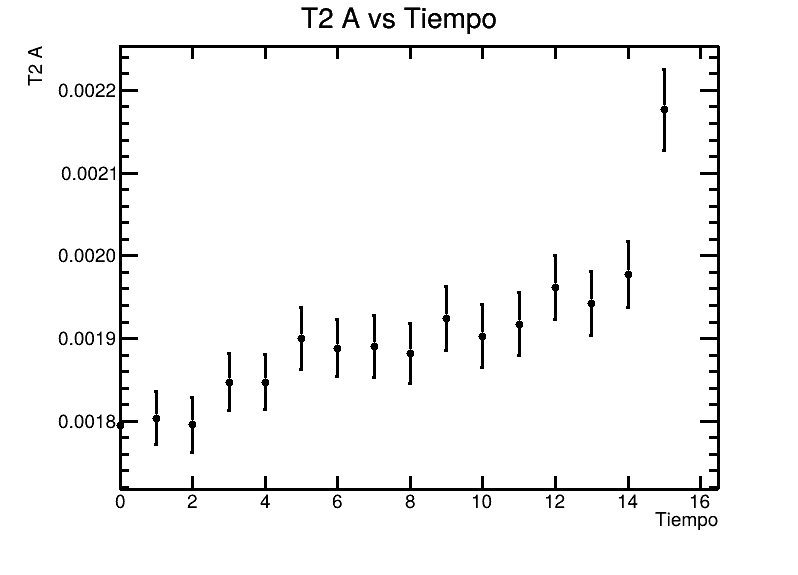
\includegraphics[width=.4\textwidth]{Chapter3/T2A_vs_tiempo.png}

    \caption{Evolución de los parámetros en función del tiempo.}
    \label{fig:T1F_vs_tiempo}
\end{figure}

%\begin{figure}[h!]
 %   \centering
  %  \caption{Evolución de $T2A$ en función del tiempo.}
   % \label{fig:T2A_vs_tiempo}
%\end{figure}

\newpage

Las gráficas obtenidas permiten evaluar la consistencia del modelo matemático utilizado para el ajuste de los datos. Si los parámetros $T1\_frac$ y $T2A$ muestran una evolución estable a lo largo del tiempo, esto sugiere que el modelo es robusto y capaz de capturar adecuadamente las características del afterglow en diferentes condiciones experimentales. Por otro lado, fluctuaciones significativas en los parámetros podrían indicar la necesidad de ajustar el modelo o considerar factores adicionales que no han sido incluidos en el análisis inicial.\\

En resumen, el análisis de la evolución temporal de los parámetros del modelo proporciona información valiosa sobre la dinámica del afterglow en el detector CMS. Estos resultados son fundamentales para garantizar la precisión de las mediciones de luminosidad y para mejorar la comprensión de los efectos que influyen en la detección de partículas en el LHC.\\


